\documentclass[a4paper,10pt,twocolumn,preprint,3p]{elsarticle}

\usepackage[latin1]{inputenc}
\usepackage{amssymb}
\usepackage{graphicx}
\usepackage{amsmath}
\usepackage{url}
\usepackage{multirow}

\journal{Expert Systems with Applications}

\begin{document}

\begin{frontmatter}

% first the title is needed
\title{Comparing individual representation and evaluation for automatic rule extraction using GP in a BYOD scenario}

\author[ugr]{Paloma De las Cuevas}
\ead{palomacd@ugr.es}
\author[uca]{Pablo Garc\'{\i}a-S\'anchez}
\ead{pablo.garciasanchez@uca.es}
\author[ugr]{J.J. Merelo}
\ead{jmerelo@geneura.ugr.es}
\author[isgt]{Zeineb Chelly}
\ead{zeinebchelly@yahoo.fr}

\address[ugr]{Department of Computer Architecture and Computer Technology, ETSIIT and CITIC \\
\url{http://citic.ugr.es} University of Granada, Granada, Spain. Tel: +34958241778. Fax: +34958248993}
\address[uca]{Department of Computer Engineering, School of Engineering \\
University of C\'adiz, Spain.}
\address[isgt]{LARODEC, Institut Sup\'erieur de Gestion de Tunis, Tunisia.}


\begin{abstract}
The constant improvement in the computational abilities and features
of personal devices has inspired the creation of the ``Bring Your Own
Device'' (BYOD) concept in the corporate world, making the companies to
create policies geared towards enabling these devices as company tools. 
This philosophy grants
employees the right to bring and use their personal devices at
the company premises, on virtual private networks, or otherwise, while
on company work. Despite the significant advantages of this policy
such as reducing overheads and increasing work productivity, 
the
access to the internal network and the assets it holds by these personal
devices, whose corporate control is forcefully limited, exposes the companies to
security threats such as leak of confidential data and access by
unauthorised users. 
To handle these kinds of threats, we propose a way of detecting and controlling abnormal user
access by establishing a policy based on classification rules that allow or deny an action, and mainly focused on having the less false positives as possible. Our
approach to address the problem of automatically obtaining classification rules to improve BYOD security uses Genetic Programming (GP), since GP is 
capable of discovering of novel and interesting threat classification
rules, with the additional feature of presenting the new rules in an
easily understandable way. % These rules are a re-formulation of the
                           % old rules set by the CSO. They are not totally new - JJ
We obtain good dataset coverage 
after the simulation results over real data, and after testing
different fitness functions and configurations in the way of coding the individuals.
Through these comparisons, we can establish a proof of concept to demonstrate the viability, effectiveness, and applicability of the GP approach, in certain conditions, to the BYOD security context for the automatic discovery of rules. 
\end{abstract}


\begin{keyword}
Bring Your Own Device, Security, Corporate Security Policy, Genetic Programming, Rule Extraction. 
\end{keyword}

\end{frontmatter}


\section{Introduction}
\label{sec:intro}

The fast pace of introduction of new technologies has led modern computing to undergo
several outstanding transitions in a short period of time. Modern
computing has moved over time to smaller, more reliable, and faster
high-tech devices such as smartphones, laptops, and tablets. The use of
these technologies in several forms is progressing, and has led to the
form of use known as the ``Bring Your Own Device'' (BYOD) concept or
philosophy. 
Since its first appearance in research
\cite{ballagas2004byod} as a way to name the interaction between
people's devices and a public display, such as art or advertising, it
has become a very popular practise, integrated into companies
\cite{thomson2012byod} and even schools \cite{song2014bring}.  

In the corporate world, the BYOD
practice refers to allowing employees to use their
personal laptops, smartphones, tablets, and other mobile devices
for work-related tasks, but not necessarily while being in the workplace. This has many
advantages \cite{singh2012byod}; among them we mention saving costs --
since the company saves money on high-priced devices that
it would normally be required to purchase for their employees --, and
increasing flexibility and worker productivity as employees will not
be asked to haul around multiple devices to satisfy both their personal and
work needs, having everything they need in one device anytime and
anywhere. 
Other advantages are tied to the increase of worker satisfaction, attracting the best candidates, and the increase of engagement in the workplace and after hours \cite{singh2012byod}. 

%These advantages have made BYOD policies gain traction in the education
%sector with an increasing number of schools around the world choosing
%to implement their own BYOD policies. % reference!!! - JJ
% Also I don't see the point. Where do you want to bring this argument to? - JJ
% Ok, maybe we talk too much about BYOD at schools when we use company
% BYOD data, but it's true that schools are environments in which
% policies should be enforced too, right? Or can be applied in another
% way... So, what can we do? To create a section at the end called
% "other applications for our framework", for example? Or just mention
% it, reducing what's written now, and that's all?
% I would go for just mentioning it, because issues are much
% different. What company "assets" are we protecting here? - JJ
%In such environment, BYOD (also called Bring Your Own Technology) refers to a technology model that
%allows students to bring their own devices to school for learning in
%the classroom \cite{sangani2013byod, song2014bring}. The adoption of BYOD in schools
%is supported by the fact that technology plays a leading role in
%pupils/students' everyday lives and should, therefore, be an integral
%part of their learning. However, for most schools it is financially
%unsustainable to provide every student with the most appropriate
%up-to-date device. BYOD is therefore considered an attractive,
%cost-effective alternative, provided that many students usually own
%devices that are superior and more up-to-date than those available in
%schools. BYOD at schools has several benefits as well such as
%personalising learning experiences, encouraging students' independent
%learning, and promoting anytime, anywhere learning opportunities. % and this is important to know because... - JJ

However, there exists a big disadvantage concerning security, since
potentially unsecured devices from unaware users might interact with
important company assets. Therefore, the main issue in the adaptation to a BYOD scenario is to obtain a high level
of security, while maintaining user privacy \cite{miller2012byod}.
Clearly the uncontrolled access to internal networks by the
personal devices, for which companies have control limits
due to privacy concerns \cite{miller2012byod}, exposes the companies to security risks such as data
leakage, improper decommissioning, phishing that is focused on a
specifig group or company\footnote{Also known as \textit{spear
    phishing}.}, 
surveillance, and many
other possible threats\cite{lennon2012changing}. These threats have become the
companies main security concern, which makes a challenge to
assure a compromise between pushing personal devices towards
professional use while coping with their own stringent and complex
security requirements. This trend is inevitable as enterprises are
faced with questions of whether and how to manage this situation \cite{thomson2012byod}; and
thus every department must be involved in establishing security
policies and procedures to minimise the company's risks.

To this end, the Corporate Security Policies (CSPs) \cite{Kaeo:2003:DNS:1201807}, 
approved by the company's Chief Security Officer (CSO) are the core at
the  identification of threats and the construction of a set of security rules. The description of these jobs include protecting
company assets by defining permissions to be considered for every
different performed action inside or outside the company's work
space, and eventually coming from the employees personal
devices. Nonetheless, CSOs build the set of CSPs based on their
expertise, and as such, they have the limitation of not knowing every
possible combination of events that might lead to a dangerous
situation. 

The aim of this paper is to propose a novel technique for extracting
inference rules from past behaviour instances 
that might help the CSO in a BYOD environment in the definition and refinement
of security policies that, eventually, classify an upcoming
event or user action as permitted or not permitted. The objective, thus, is to obtain a way of correctly classifying the most incoming events as possible, avoiding mostly the false positives \cite{pietraszek2005data}. By false positives, we mean that events that must not be permitted should never receive an ``ok'', that is, a GRANTED. 
This could be used
in two different scenarios. In the first one a CSO has hand-coded a set of security
policies and wants to simplify or generalise them. The second scenario 
would simply dispense with rules and have the CSO decide, by hand, which
particular events wants to grant or deny access, and have a system such
as the one described in the paper generate a set of security policies
by creating a set of rules from particular events. 
The main objective in both scenarios is to create a reliable rule set
which is able to cover every new situation that may be a threat;
allowing the system to go beyond the limited set of known pre-defined
rules. Additionally, this feature can be used as ``reverse
engineering'', so that the rules initially made by the current or
former CSO are found in the solution along with additional ones. In
order to have the space of possible policy rules be as wide 
as possible, it is necessary a technique that explores the rule space
efficiently and with the least assumptions about rule structure.

This is why we have decided to use Genetic Programming (GP) for dealing with the problem of
discovering novel, interesting knowledge and rules from large
amounts of data \cite{freitas2002data}, given that the up-to-date approaches are based in general pre-defined of manually defined rules \cite{ali2015analysis}. Considered part of the so-called \emph{Evolutionary
  Algorithms} \cite{back1996evolutionary}, GP is an optimization
technique inspired by natural evolution. One of the advantages of GP is that by making the
solutions to a problem internally encoded as trees, they themselves can be
seen as decision tree classifiers \cite{safavian1990survey} and can be expressed as a set of rules.

To the best of our knowledge, there is still not a tool that helps CSOs in
developing new security rules via GP, even as this method has been
indeed applied to classification, as described by Espejo et al. in
\cite{espejo2010survey}. In fact, their survey theoretically supports our
decision of applying GP to obtain security rules in a BYOD
environment.

In our case, the assigned classes, or leaves of the tree, would be ``allow''
or ``deny'', acting over a certain incoming event; whilst the nodes
are the conditions that have to be met to apply the action. Taking
this into account, GP can be used to generate these classification
trees, optimising an objective function called {\em fitness}. In this case the
fitness can be defined as the accuracy of a rule or set of rules, being this the most
used metric in classification \cite{witten2005data}, along with the
classification error. But since there are other metrics that influence in
``how good'' a rule or a set of rules is, such as the depth of the
created tree, the number of nodes it has, or the obtained false positives
\cite{back1996evolutionary}, it would be of convenience to use them in
the definition of the fitness. 

Our proposed GP framework is capable of performing an automatic discovery
of classification rules from the BYOD context data, obtaining good fitness values, and presenting the
rules in a way that is helpful for a CSO. We demonstrate so by using
the developed framework with a real-world dataset, and comparing two
ways of coding the individuals -- as a set of rules, or as a single
rule -- so that we are able to choose the best approach for our system. We make this comparison because while obtaining a set of rules as a solution is computationally expensive due to the need of longer evaluations, to present and evaluate a single rule not taking into account how it interacts with what the others cover \cite{freitas2002data} can lead to massive overlapping. Hence, we must study their accuracy despite of their advantages and disadvantages. In addition, we choose the most appropriate (fastest to converge and with best value) fitness after comparing the use of a most simpler one that only measures the accuracy, and a complex one which takes into account the complexity of the individuals. Finally, we propose the approach with the best performance in terms of best coverage over a validation set. 

The rest of the paper is organised as follows. In Section
\ref{sec:SotA} we give an overview of the advances in GP applied to
rule evolution and its applications; then, Section
\ref{sec:methodology} describes the proposed methodology, depicting
the problem this work tries to solve and describing the available
dataset and the proposed GP framework. The experimental setup, as %Pablo: I've seen more times the "setup" definition rather than "set-up"
well as the different set of experiments that have been carried out
are also described in that section. Section \ref{sec:gp} shows and discusses the
obtained results from the application of GP to security rules
extraction and, finally, the conclusions of this work along with some
suggestions about how to continue our research are given in Section
\ref{sec:future}.   

\section{Related Work}
\label{sec:SotA}

Since BYOD policies started to appear in companies' day-to-day policies  a lot
of research has been done about the advantages and disadvantages of
this approach \cite{singh2012byod}, as well as about how to properly implement it in order to
respect privacy while trying to secure the resources \cite{scarfo2012new, ali2015analysis, de2015corporate}.
These issues can be approached in different ways; Scarfo
differentiates in \cite{scarfo2012new} two main ones: allowing the
device to connect via desktop or application virtualisation, meaning
enough control to avoid employee's devices monitorisation; or allowing
the company to control devices
via Mobile Device Management (MDM), which has to be legally agreed
with the employee. %Mention disadvantages: the company has to provide
                   %a virtualization platform and pay for cloud
                   %resources, or the employee has to allow the
                   %company to control its own device, which
                   %eventually dispels two of the advantages of BYOD
                   %policies: low overhead cost and preservation of
                   %privacy. (something like that). 
 Ali et al. expand from Scarfo's study in
\cite{ali2015analysis} reviewing both BYOD access control
 and security models. The authors further distinguish
between MDM and Kernel Modifications inside the security models, and
conclude with the description of a proposed model which combines most
of the reviewed solutions, i.e. MDM and Virtual Private Network (VPN)
access together with an encrypted container for the accessed
information depending on the level of restriction. However, from all
the papers in \cite{ali2015analysis} claimed to enforce policies, only
in \cite{rhee2013high} the authors actually describe how the policies
are enforced by describing which data is monitored. In any case, none
of the papers mention the application of GP to the enforcement of the
security policies, but other techniques such as the implementation of
blacklists to avoid the installation of forbidden applications, or
whitelists to allow only certain ones. These techniques can be useful
with respect to the implementation of already defined security
policies, but our method allows to discover new security policies,
which in the case of black and white lists, can evolve them to include
new and/or malicious applications. 

Research in BYOD has been accompanied by innovation in products released
to help companies implement or streamline the process of adoption of the BYOD
concept. In \cite{de2015corporate} there is a description of the
market solutions that the main manufacturers have developed to such
purpose. The level of security and privacy preservation offered by
these applications is different depending on the solution.
None of the reviewed solutions, but one, seem to offer a dynamic
creation of rules in the database used for incident detection. Our work is part of the project called MUSES, as one of its aims is implementing rule inference using GP, among other techniques. In this work we extend the description of the
rule inference process through GP, as well as the details of its implementation
and the results after applying it to a set of data gathered during the project. 


Previous papers have commented on the issue of using quality data to obtain accurate and valuable extracted knowledge, which is specially difficult when dealing with datasets taken from real world problems, where the sensors cannot work properly at a certain time.
To avoid this, researchers have advanced the state of the art in the precision of the
devices. For instance, in \cite{rios2015mobile}, the authors focus on
the importance of having an accurate measure of the location of the
devices. Although their approach seems to encroach upon employees'
privacy, they implemented a mobile information system for BYOD
adaptation, and tested it in both Android and iOS devices. The authors
concluded that the efficiency of their system, along with the
possibilities of the hardware in the devices, results in a location
error of less than 50 meters with a 95\% confidence level. These
promising results allow the companies to use the location of their
employees to apply certain security policies. In our case, an accurate detection of the location could be used to obtain more information about the happening event, and that could increase the classification accuracy. 

%Another barrier to obtain good quality knowledge discovering are datasets that present imbalance, because they normally bias the elaboration of classification rules or trees towards the majority class - the class with higher representation in the dataset - \cite{japkowicz2002class}. In this sense, solutions can be found in literature in order to reduce the bias while performing classification tasks, such as in \cite{chawla2005data} and \cite{sun2009classification}. However, as we have center our proposal in GP, we have studied Bhowan et al.'s work in \cite{bhowan2012developing}, where they present a comparison between many different types of fitness functions, testing on various unbalanced datasets, with different minority-class/majority-class ratios.

Another issue is the adequate way to prepare the extracted data. And even though a lot has been advanced in preprocessing techniques in order to work with quality and accurate data \cite{han2011data}, still there is room for research in the discovery of new rules from real world data. With respect to classification applied to real world data in order to obtain classification rules, Espejo et al. review in \cite{espejo2010survey} three papers which use GP for classification with
communications data, but mainly for intrusion detection and e-mail
spamming. Thus, the works they review have applications in
all fields but not exactly the one we focus on here. In \cite{Tsakonas2004195} the authors also extract rules with \textsc{IF \ldots THEN} structure through GP, although for medical purposes. Futhermore, Alex A. Freitas deeply studied the application of GP to Data Mining (DM) in \cite{freitas2002data}, providing the necessary knowledge and guidelines to design a GP framework for DM applications. Also, in \cite{DeFalco2002257}, a system which discovers
rules for the PROBEN1 databases via GP is described and a new fitness is introduced. PROBEN1 \cite{prechelt1994proben} is a collection of datasets from real world problems meant as benchmarks for the application of classification techniques. As happened in 
the survey of Espejo et al., from six of the databases inside PROBEN1 and
analysed by these authors, none is related to security. However, the
authors' proposed fitness is indeed of interest for this research, and
as such we compare the performance or our algorithm using two
different fitness functions: the more classical approach that measures
only the correctly classified instances (accuracy); and De Falco's et
al. \cite{DeFalco2002257} suggestion, also taking into account the
complexity of the solution.

%Once again, this paragraph does not follow the previous one. Maybe
%move it one paragraph up, where you are talking about proper training
%data. 
Finally, the lack of BYOD-related security databases is a hindrance for the
proliferation of research in this field. As seen, there actually exist
a number of datasets related to malware, e-mail spamming, or URL
requests \footnote{http://www.secrepo.com/}, but none about the use
that people make of their smartphones. This situation clearly exists
due to privacy considerations. Miller et al. \cite{Miller201253}
firmly state that the issue of privacy is even more important than the
security issue, although it does not receive the same
attention. Furthermore, when the MDM solution is described in
\cite{ali2015analysis}, the authors mention the privacy concerns the
employees may have due to the processing that the company makes over
all their behavioural data. And even after anonymising the resulting
dataset, one can still, in certain cases, identify a user of the
company the data comes from by processing the data. If this principle
cannot be guaranteed, the data should not be released
\cite{boillat2014handbook}.
% This paragraph is not the state of the art in your methods or
% problem. You are eventually not releasing data, either. Suggestions:
% 1. Eliminate it
% 2. Eliminate it and add a note in the "future work" section saying
% that future data sets will be released by ourselves.
% As above, erase when accepted or rejected - JJ

\section{Methodology}
\label{sec:methodology}

As previously highlighted, the main idea behind corporate security
policies, which are defined by the CSO, is to build a basic, fixed,
and well defined set of rules, which take the form of \textsc{IF
  \ldots THEN} clauses. By applying them, the company system decides if certain conditions are met in order to allow or
deny access to an asset, whether is from the company or is accesed from it. 
Therefore, these rules can be visualised as the actions, taking place in a precise environment, being classified as
allowed or denied. In this sense and while facing a security breach
from a BYOD system, the set of rules will be tested looking for
matches between the access' characteristics and the rules' premises --
the conditions expressed in the IF part, also known as the description
of the rule \cite{DeFalco2002257}. If it matches then the decision can
be made, by checking the conclusion part of the rule, which comes
after the THEN and indicates the class \cite{DeFalco2002257}, either
by allowing or denying employees' access to non-confidential
 or non-certified data, for example. However, it is important to
 mention that the companies'  set of security rules defined by the CSO is
 based on known and previously recognised accesses and thus it cannot
 cover the whole, safe and unsafe, search spaces. Therefore,
 there is an urgent need to develop a system capable of discovering a
 more reliable rule set which should be able to cover every new
 situation that may be a threat. Hence, allowing the company security
 system to go beyond the limited set of known, pre-defined rules.  % This rather belong to the introduction - JJ
 % (Paloma) The whole paragraph?
% What do you think? - JJ

Our proposed solution is based on a novel GP framework dedicated for
the BYOD context and capable of performing an automatic and wider discovery of classification rules. More precisely, our GP based framework will, first, extract all the possible values of every attribute in the data at hand and then make the GP algorithm evolving. 
Specifically, in this context, we have decided to follow the more
conventional approach in Genetic Programming, the Pittsburgh approach
\cite{freitas2002data}, meaning that each individual is seen as a set
of rules. However, in this work we have also implemented the Michigan
approach, where every indidual is a single rule. The aim of having these two different implementations is to choose the most efficient, in terms of time to find the solution, best fitness, accuracy in the validation phase, and readability.

The last step would be to present the rules -- solution -- to the CSO of the company and tune the algorithm according to the decision of
finally including or not the set of rules in the main security
policy. The description of the used data and further explicit details
about our proposed solution are given in what is next.

\subsection{Available Data}
\label{subsec:data}

 The set of used data has been gathered from the trials that were performed
 during the development of an FP7 European Project, called MUSES
 \cite{DBLP:conf/sac/MoraCGZJEBAH14}. In these trials, a group of
 users tested a smartphone and PC application meant for securing a
 BYOD environment. The application generates warnings when the users
 act in a dangerous way. Technically, these warnings are triggered by
 a set of initial and pre-defined rules, so that when certain
 conditions are met in an ``event'' (an action performed by a user),
 the corresponding action could be allowed - nothing happened - or
 denied, where a warning appears explaining the rule that the user did not comply with and how to perform the action in a more secure way or environment.

The dataset contains a set of these ``events'' from which a number of attributes (variables) have been extracted or are given by the application itself. User data has been also extracted but anonymised, in the sense that from all the attributes extracted from the user actions, the username is not included as a variable to build rules with. The attributes can be classified in different ways; one of them is based on whether they are directly read from the application or inferred after processing the read data. Therefore, we distinguish between:
\begin{itemize}
  \item Attributes given by the tested application: these attributes
    are related to the type of the event (action), its timestamp, or
    the application which originated the event, among others. 
  \item Attributes inferred from the information in the database: the information given by the aforementioned attributes, along with the rest of information already existing in the database, helps inferring other attributes. These are, for instance: all extra information related to the origin, like the user position in the company or the device Operating System; the configuration of the device, such as WiFi or Bluetooth being enabled; and even lexical properties of the user password, in order to avoid storing the password itself or using it for classification or rule generation.
\end{itemize}

The trials had a duration of five weeks, and a total of 
153270 events were registered in the database. We filtered those events that did not imply access to assets, meaning that they were not useful for
knowledge extraction purposes, such as events of \textit{log in},
\textit{log out}, or \textit{restarting the server}.
The remaining was a 35\% (53296 instances) of the total, and were considered as \textit{important}
because they did contain information about user actions such as
opening files or sending emails in a certain connection environment,
changing security properties, or installing apps. Altogether, there
are 38 attributes, plus the class, which can take two possible values:
GRANTED or STRONGDENY. 

%With respect to the balance between the classes, the dataset is
%unbalanced with the following ratio: 49289 instances are labelled as
%GRANTED and 4007 are labelled as STRONGDENY. % If what follows this
                                % full stop, that is, nothing, is what
                                % you are going to do about it, it is
                                % better to just not mention it. It
                                % begs the question by rev. number 3:
                                % How are you addressing this
                                % unbalance in the paper? Will that
                                % affect the choice of training
                                % methods or the result? Please repeat
                                % experiments, ALL of THEM, to address
                                % this unbalance - JJ

\subsection{Proposed Solution}
\label{subsec:solution}

As previously highlighted, in this work we propose a system which is
able to process a set of user actions that have been allowed or denied
based on initial, simple rules, and discover new rules through GP by exploring
the whole space of possible combinations among the attribute
values. The coding of the individual might take two approaches, named \textit{Pittsburgh} and \textit{Michigan}
\cite{freitas2002data}.

The Pittsburgh uses GP to create an individual tree that
model a set of different rules, given that the problem can be seen as
a 
classification one and therefore the model can be a decision tree
\cite{safavian1990survey}. Then, the generated tree is a binary tree
of expressions formed by two different types of nodes:

\begin{itemize}
\item {\em Variable}: it is a logical expression formed by a prefix, a
  name, an operator and a value. It is the equivalent to a
  ``primitive'' in the field of GP \cite{back1996evolutionary}. The
  operators depend on the type of variable, being \{=$>$\} (an arrow, as in ``takes the value of'') in the
  case of categorical attributes, \{=\} for binary attributes, and \{$<$, $<=$,=,$=>$,
  $>$\} for numeric ones. At the same time, the prefix can be \{AND,
  OR\}, and NOT can appear before these. \\ %Pablo: removed the "randomly" word because it may confuse the reader
    Examples:
   \begin{math}
     \left \{
   \begin{array}{l}
     \texttt{password\_length<5} \\
     or \\
      \texttt{event\_level=>COMPLEX\_EVENT}
   \end{array}
   \right .
   \end{math}
\item {\em Action}: it is a leaf of the tree and therefore, a ``terminal'' state. Each decision is the result of applying the rule, so it is limited to two terms which are \texttt{GRANTED} or \texttt{STRONGDENY}. Only one leaf must hung from a parent (variable) node.
\end{itemize}

Rules are constructed starting from each leaf of the tree and iterating to the upper parents, or variables, reading their data as string. Therefore, the number of rules of the set produced by the tree is equal to the number of its leafs. It is worth mentioning that some rules might have contradictory conditions inside them during the evolution. This is not a problem because those rules will not cover any instance and thus they will not contribute to the fitness value. 

The second approach tested, called Michigan approach, assigns a single
rule to every individual. In this paper we have expressed the rule as
a list of conditions, with a fixed class, obtaining just one rule per
execution. That means we are not using GP in this case, because the
generated individual is not a tree, but a vector, so we are applying a
regular Genetic Algorithm (GA) instead. Therefore, in order to cover
all classes, the algorithm has to be executed once for each class; in
our case, GRANTED, allowed actions, and STRONGDENY, for the denied
actions. 

Indeed, each approach has its advantages and disadvantages. The Pittsburgh approach allows to directly obtain a set of rules able to classify instances of every existing class, meanwhile Michigan approach's solution is coded as a single rule, so that we obtain as many rules as classes are defined. The possibility of having many rules for every class instead of just one, more general, per class might seem to better help the CSO in detecting specific dangerous situations.
At the same time, obtaining a set of rules as solution is more
computationally expensive due to the need of longer
evaluations. Lastly, to evaluate a single rule not taking into account
how it interacts with what the others cover \cite{freitas2002data}
can lead to massive overlapping with the consequent loss of
efficiency. 

With respect to the variables, both approaches use three different types, 
described as follows \cite{witten2005data}:

\begin{itemize}
\item {\em Binary Variable}: those with a boolean value, for instance, variables that are related with the device services switched on or off and important features such as the device having or not an antivirus installed. 
\item {\em Categorical Variable}: the ones with nominal values, where it is defined a list with the possible values it may have, in order to randomly pick up one in the creation of the rules. 
\item {\em Numerical Variable}: those with a numerical value, for which both maximum and minimum values are specified. 

\end{itemize}

Table \ref{tab:variables} details the variables, for each type, that have been used in the GP in order to create the rules. In addition, we differentiate between those variables that are BYOD specific, and those that come from the context. A variable that is BYOD specific means that its value strictly depends on the employee owning the device or being provided by the company, such as the device OS, if the device has been rooted, or the password length the user has configured. The same way, a variable that is the same no matter who owns the device, for instance, the user role or the type of the action (event) performed, we say is context specific.

\begin{table}
\begin{center}
	\resizebox{8cm}{!}{
\begin{tabular}{|l|l|l|l|}
\hline
Variable type                & Variable Name          & BYOD & Context \\ \hline
\multirow{8}{*}{Binary}      & BluetoothConnected     &               & \checkmark       \\ \cline{2-4} 
                             & DeviceHasAccessibility & \checkmark    &                  \\ \cline{2-4} 
                             & DeviceHasAntivirus     & \checkmark    &                  \\ \cline{2-4} 
                             & DeviceHasPassword      & \checkmark    &                  \\ \cline{2-4} 
                             & DeviceIsRooted         & \checkmark    &                  \\ \cline{2-4} 
                             & MailHasAttachment      &               & \checkmark       \\ \cline{2-4} 
                             & WifiConnected          &               & \checkmark       \\ \cline{2-4} 
                             & WifiEnabled            &               & \checkmark       \\ \hline
\multirow{8}{*}{Categorical} & AssetConfidentialLevel &               & \checkmark       \\ \cline{2-4} 
                             & DeviceOS               & \checkmark    &                  \\ \cline{2-4} 
                             & DeviceOwnedBy          & \checkmark    &                  \\ \cline{2-4} 
                             & DeviceType             & \checkmark    &                  \\ \cline{2-4} 
                             & EventLevel             &               & \checkmark       \\ \cline{2-4} 
                             & EventType              &               & \checkmark       \\ \cline{2-4} 
                             & UserRole               &               & \checkmark       \\ \cline{2-4} 
                             & WifiEncryption         & \checkmark    &                  \\ \hline
\multirow{2}{*}{Numerical}   & DeviceScreenTimeout    & \checkmark    &                  \\ \cline{2-4} 
                             & PasswordLength         & \checkmark    &                  \\ \hline
\end{tabular}
}
\caption{A list of the variables that have been used to generate the
  rules. Those variables that are BYOD specific are also specified.}
\label{tab:variables}
\end{center}
\end{table}

At the end of the process, either as part of a set of rules or just being a single rule, they can be presented as follows:

\begin{verbatim}
device_has_antivirus=false AND
password_length<5 AND
user_role=>Administration OR
device_is_rooted=true THEN=STRONGDENY
\end{verbatim}

Rules presented in this way offer good readability which is key to understand the relation between the attributes and how the described situation may, or may not, be dangerous. In the example, the system would have inferred that an action from a device without antivirus, a short password, and rooted or belonging to an administration employee, should be denied.
% (Paloma) Shall we explain what a rooted device is?
% You should rather say what is the relationship between these rules
% and the original rules - JJ
% Still can't see why you need to train several times. Can't you just
% train once and obtain the best individuals at the end of training? -
% JJ
% (Paloma) No, you train for every fold.

\subsection{Choosing a suitable fitness}
\label{subsec:chossingfitness}

In the application of GP to classification
the most used metric to evaluate the individuals, i.e. the fitness function, is the accuracy
\cite{espejo2010survey}. The accuracy is normally obtained as the
ratio of the correctly classified instances among the total of
instances. %However, in our particular case, there is a strong
           %asymetry between FP and FN. That is why... - JJ
           % (Paloma) ????
% If you are going to mention imbalance between FP and FN this would
% be the place to introduce it. 
% (Paloma) But why?? We are introducing the concepts, is it normal then to directly talk about the results so soon? :\
Witten et al. use in \cite{witten2005data} the
concepts of true positive/negative and false positive/negative. The
first refers to the correctly classified instances, and the latter are
those instances that should be negative (positive) but are classified
as positive (negative), therefore they are false positives
(negatives). Using this nomenclature -- true negative (TN) and true positive (TP) --, a fitness function defined for
accuracy would be expressed as follows: 

\begin{equation}
\label{eq:accuracy}
f_{Acc} = (TP + TN) / T_{tr}
\end{equation}

This kind of fitness has to be maximised, given that the ideal value
of $f_{Acc}$ is the whole training dataset, $T_{tr}$. Equation \ref{eq:accuracy} has the 
advantage of not being computationally expensive, but it does not
penalise the badly predicted instances (false positives and
negatives), which in security environments such as this one can be
very harmful. Furthermore, a false negative would mean that the system denies an event that should be allowed, but the worst case scenario is having a false positive, when a dangerous event is classified as allowed.
To this end, in \cite{witten2005data} the authors define the coverage as:

\begin{equation}
\label{eq:coverage}
C_{ind} = TP + TN - (FP + FN)
\end{equation}
Additionally, to take into account the complexity of the individuals,
either they are a rule or a set of rules, in \cite{witten2005data}
they introduce a measure of the generated trees or list size by this
expression: 

\begin{equation}
S_{ind} = N_{nodes} + depth
\end{equation}

Where $N_{nodes}$ is the number of nodes of the tree (or elements in a list), and $depth$ is the tree depth. So that combining $C_{ind}$, $S_{ind}$ and introducing an $\alpha$ variable inside [0, 1] to tune up the degree of allowed complexity, the problem becomes now a matter of minimising this formula:

\begin{equation}
\label{eq:complexFitness}
f_{CS} = (T_{tr} - C_{ind}) + \alpha S_{ind}
\end{equation}

Therefore, in our experimental section we are going to compare both
$f_{Acc}$ and $f_{CS}$, with different  alpha values, to check two statements:

\begin{itemize}
	\item How they influence in the number of evaluations taken to find the best solution.
	\item Which fitness function contributes best to obtain the less FP and FN as possible.
\end{itemize}

And finally decide which fitness function offers, taking into account these measures, the best performance. 

% And, eventually best results are obtained for alpha = 0. So depth
% really does not matter. That can be introduced in different ways
% that do not affect fitness, such as selective pressure - JJ

% Please note also that you are not making any reference to the
% STRONGDENY and GRANTED classes you include in the tables. 

\subsection{Experimental Setup}
\label{sec:experiments}

Once the methods to compare have been explained, the rest of the experimental setup is described.

The configurations that will be compared involve two different encoding of individuals (Pittsburgh tree individuals vs. Michigan list individuals), two types of fitness ($f_{CS}$ and $f_{Acc}$), and three different values for $\alpha$ in the case of $f_{Acc}$.

With respect to the GP parameters, different decisions for experimental design have been taken into account. 
First, sub-tree crossover and 1-node mutation evolutionary operators have
been used, following our previous works that have used these operators
obtaining good results \cite{EvoStar2014:GPBot}. In this case, during the
mutation operation, there is a 50\% of probabilty to change the complete variable (prefix, name, operator and value) or only the value. A population of 32 individuals and a 2-tournament selector for a pool of
16 parents have been used. These parameters have been also previously used in previous GP works \cite{EvoStar2014:GPBot}. Table \ref{tab:parameters} summarises all the parameters used.

\begin{table}
\begin{center}
\resizebox{8cm}{!}{
\begin{tabular}{|c|c|}
\hline
{\em Parameter Name} & {\em Value} \\\hline
Population size & 32 \\\hline
Crossover type & Sub-tree crossover \\ \hline
Crossover rate & 0.5\\ \hline
Mutation  & 1-node mutation\\ \hline
Selection & 2-tournament \\ \hline
Replacement & Generational with elitism\\ \hline
Stopping criterion & 150 generations \\ \hline
Maximum Tree Depth & 10 \\ \hline 
Runs per configuration & 10 \\ \hline
\multicolumn{2}{|c|}{{\em Compared configurations}} \\ \hline
Individual representation & Pittsburgh vs. Michigan \\ \hline
Fitness & $f_{CS}$ VS $f_{Acc}$ \\ \hline
$\alpha$ for $f_{CS}$ & 0, 0.5, and 1 \\ \hline

\end{tabular}
}
\caption{Parameters used in the experiments.}
\label{tab:parameters}
\end{center}
\end{table}

During the fitness evaluation, the generated individual is converted
into a string, which can become a single rule or set of rules
depending on the approach, as previously described. % But this is what you are going to
                           % compare. You should make a lot of more
                           % emphasis - JJ
Then, the chosen fitness is evaluated for a particular rule -- the single rule or each one inside the set -- and over the 90\% of the data.
For further reliability of the results, it is advised to perform
10-fold cross-validation \cite{kohavi1995study}, and as such the WEKA %Pablo: it is worth mentioning WEKA here? (well, in fact, I wrote this paragraph, but Paloma decides)
% (Paloma) Uhm, maybe it's not THAT necessary, but it does not bother either... i don't know xD 
Java Library \cite{HallWEKA09} has been used to generate the 10 folds
or distributions of data into 90\% training (fitness evaluation) and
10\% validation. This way, each experiment has been executed 10 times,
each one with a different distribution of data.

The algorithms have been executed in a cluster node with 16 Intel(R) Xeon(R) CPU E5520
@2.27GHz processors, 16 GB RAM, CentOS 6.8 and Java Version 1.8.0\_80.

The specific source code of the proposed method is available under a LGPL V3 License 
at \url{https://github.com/fergunet/GPRuleRefinement}, as a module for 
the framework OSGiLiath \cite{DBLP:journals/soco/Garcia-SanchezGCAG13} 
\footnote{The source code of OSGiLiath is available with the same
  license  as well, at \url{http://www.osgiliath.org}.}.


%\subsection{Results from Classifiers}
%\label{subsec:classifiers}

%\subsection{Results from Association Algorithms}
%\label{subsec:association}

%\subsection{Results from Clustering}
%\label{subsec:clustering}

%\subsection{Results from Genetic Programming}
%\label{subsec:gp}

%\section{Discussion}
%\label{sec:discussion}

\section{Results from Genetic Programming application} 
\label{sec:gp}

% A paper is a story, has a narrative. Introduce the section by
% stating where in your narrative are right now. "Remember, dear
% reader, that we wanted to compare the two proposed approaches
% because... We are going to do so right here" - JJ

As our purpose in this paper is to obtain a system which proposes to a CSO useful security rules that improve the existing ones, and present them in an understandable way, in this section we compare the results from using two fitness functions
described in Equations \ref{eq:accuracy} and \ref{eq:complexFitness}, as well as the two approaches taken -- Pittsburgh and Michigan --. In addition, an example of the individuals obtained will be presented in order to understand how the different approaches affect them, along with
their advantages and disadvantages.
Lastly, we will choose the best
approach, justifying this choice. 

% You are not examining different approaches and reporting results on
% them. You are trying to solve a problem, for which you are testing
% different approaches, and it should be very clear to you how to test
% what solution is the best INDEPENDENTLY OF THE APPROACH, so you
% might have to come up with a way of comparing solutions
% independently of the fitness you are using. At any rate, the reader
% is not interested in Pittsburgh and Michigan approaches _separately_
% but on which one yields the best solution. Boils down to: don't
% separate results, compare them, even less so in different
% subsections.

\subsection{$F_{Acc}$ vs. $F_{CS}$} 
\label{subsec:fitnesscomparison}

The aim of this comparison is to conclude which fitness function should be used, discussing the results from the point of view of convergence, and that means finding which one reaches the best value faster. To study this we have displayed the obtained fitness through the iterations for the Pittsburgh approach in Figure \ref{fig:pittsburghItvsF} and for the Michigan approach in Figures \ref{fig:michiganItvsF_allow} and \ref{fig:michiganItvsF_deny}. Figures for GRANTED and STRONGDENY classes are separated because the solution is a single rule instead of a set of rules, and therefore the algorithm has to be executed once per class. With regard to the best fitness obtained for each fitness function, they are similar in the same scope, which means that the different values of $\alpha$ in $f_{CS}$ did not present significant differences in the two approaches separately.

\begin{figure*}[h!tb]
\centering
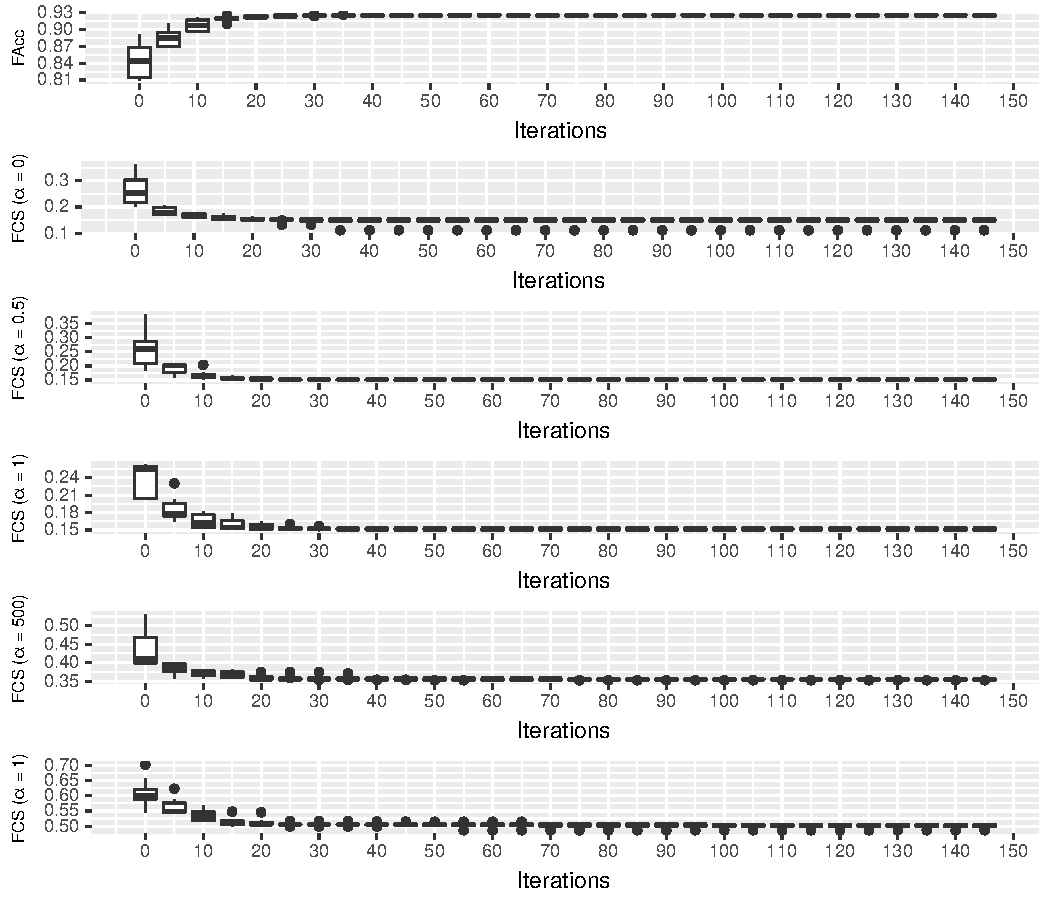
\includegraphics[width=0.8\textwidth]{img/pittsburghItvsF.pdf}
\caption{Convergence of fitness for each one of the tested fitness
  functions, and for Pittsburgh approach. Note that $f_{Acc}$ has to
  be maximised, whereas $f_{CS}$ has to be minimised.} % You know what
                                % I think about these graphs, from
                                % this one to the third. Using
                                % boxplots only makes them a bit more
                                % confusing. Boxplots should be used
                                % for comparing categories or
                                % factors. - JJ 

\label{fig:pittsburghItvsF}
\end{figure*}

For the sake of clarity, $f_{CS}$ has been divided by the maximum
value -- the number of instances for training -- it might take. By
looking at the Pittsburgh approach values in Figure
\ref{fig:pittsburghItvsF}, we show that mostly all configurations tend to converge around iteration 40, but it seems that $f_{CS}$ with
$\alpha = 0.5$ is the configuration that reaches the best solution
faster, around the 30th iteration.  

\begin{figure*}[h!tb]
	\centering
	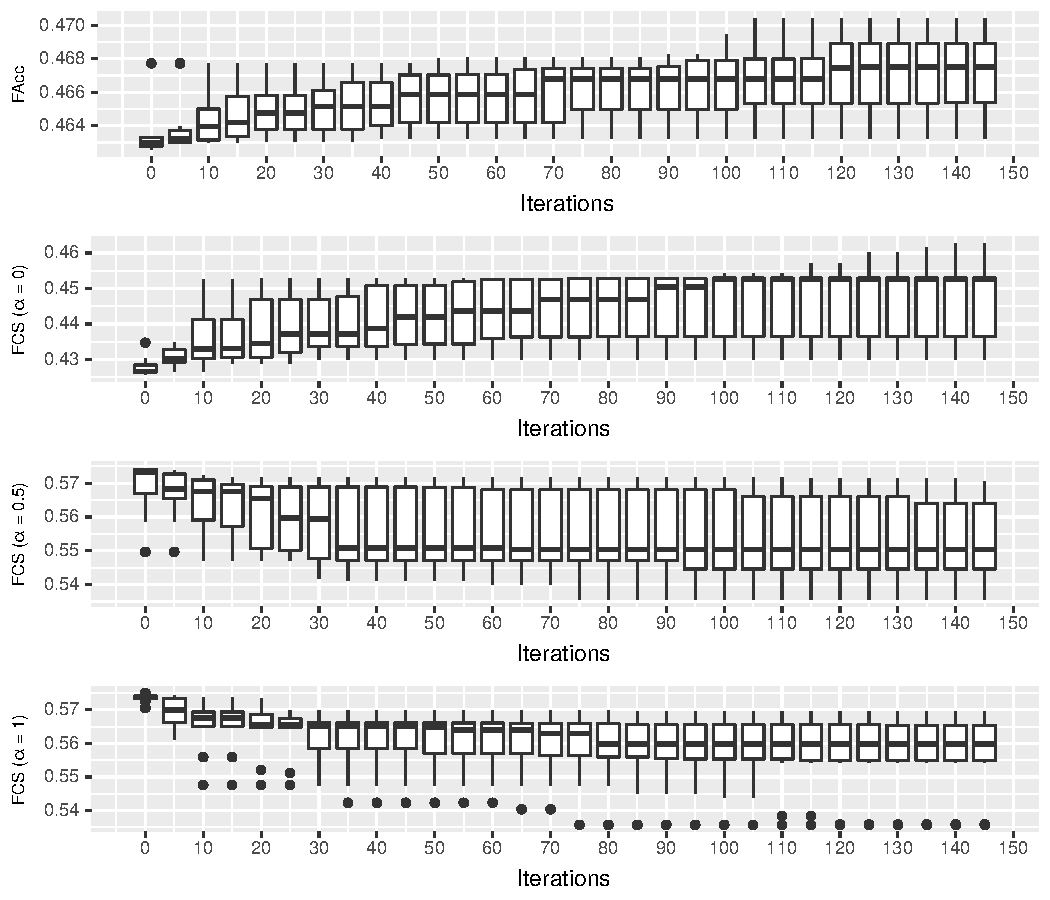
\includegraphics[width=0.8\textwidth]{img/michiganItvsF_allow.pdf}
	\caption{Convergence of fitness for each one of the tested fitness functions, and for Michigan approach being executed for the GRANTED class. Note that $f_{Acc}$ has to be maximised, whereas $f_{CS}$ has to be minimised.}
	\label{fig:michiganItvsF_allow}
\end{figure*}

With respect %Pablo: changed to "respect" because with regard was used not so long ago. Also, more respect imply a more Ali-G-ied paper.
to the Michigan approach, a higher variability is noticeable in Figures \ref{fig:michiganItvsF_allow} and \ref{fig:michiganItvsF_deny}, but in average we see that for $f_{CS}$ with $\alpha = 0$ or 1, the fitness do not converge until generation 120. The best ones are for $f_{Acc}$ and $f_{CS}$ with $\alpha = 0.5$, being the latter the one that converges faster, around the 50th iteration.

\begin{figure*}[h!tb]
	\centering
	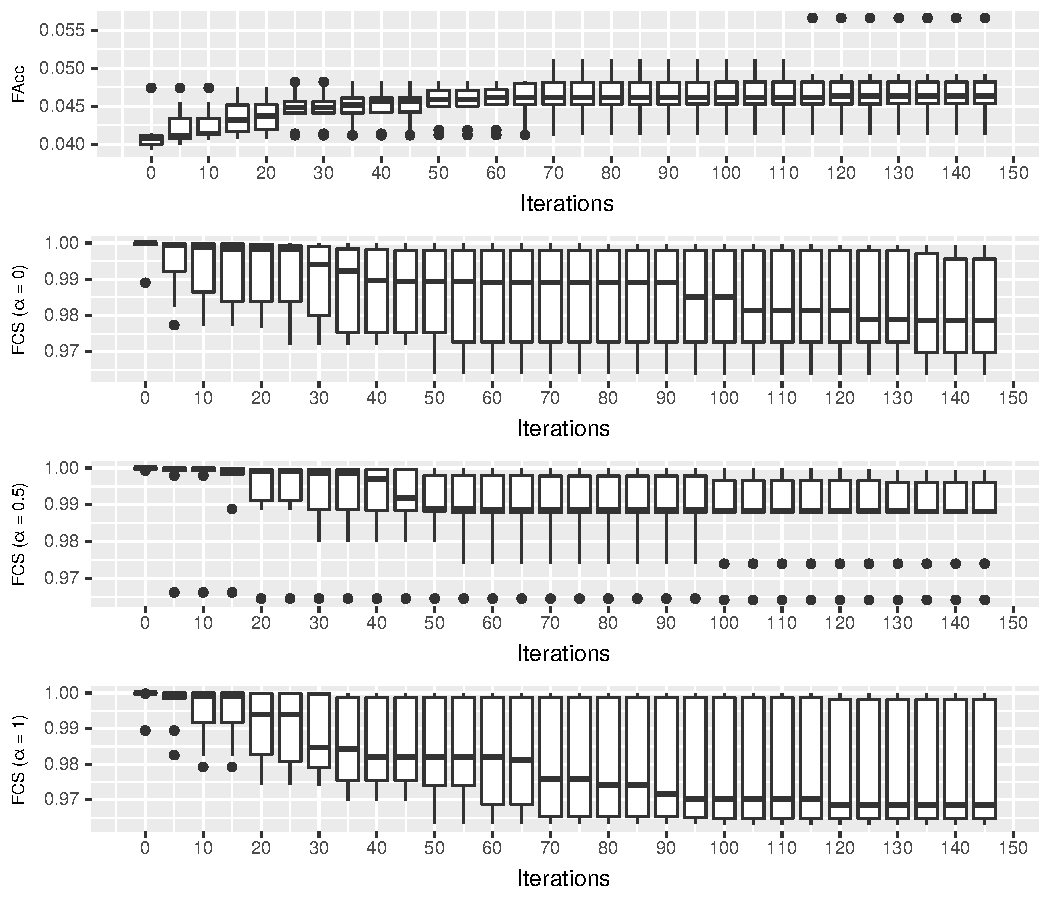
\includegraphics[width=0.8\textwidth]{img/michiganItvsF_deny.pdf}
	\caption{Convergence of fitness for each one of the tested fitness functions, and for Michigan approach being executed for the STRONGDENY class. Note that $f_{Acc}$ has to be maximised, whereas $f_{CS}$ has to be minimised.}
	\label{fig:michiganItvsF_deny}
\end{figure*}

We can advance that the best results might be obtained for $f_{CS}$
with $\alpha = 0.5$. However, there is a considerable difference between the performance, in terms of best
obtained fitness, of the two used approaches. In this way, we have to thoroughly compare them. In the next section we do so by chosing the validation coverage and the ratio of false positives and negatives as independent measurements. 

\subsection{The Pittsburgh vs. Michigan approach} 
\label{subsec:approachcomparison}

Once the variability of the obtained fitness has been studied, and
always taking into account that those values come from their
evaluation in a training subset of the data, now we \textit{validate}
the proposed approaches with a validation set, similar to the validation set used in classification problems \cite{witten2005data}. 
 The way to evaluate this is similar to Equation \ref{eq:accuracy}, but using the validation subset of the data:

\begin{equation}
\label{eq:VALaccuracy}
v_{Acc} = (TP + TN) / T_{tst}
\end{equation}

This measure will be the same independently of the approach or fitness
function has used to evaluate the individuals. Table
\ref{tab:PvsMvalidation} shows the average, best, median, and worst
results from the evaluations with $f_{Acc}$ and also $f_{CS}$. 

\begin{table*}
	\centering
	\resizebox{16.5cm}{!}{
		\begin{tabular}{llll|l|l|l|l|l|l|}
			\cline{5-10}
			&  &  &  & \multicolumn{6}{l|}{Validation measurement} \\ 
			\cline{3-10} 
			& \multicolumn{1}{l|}{}  & \multicolumn{2}{l|}{Fitness function}  & Average & Best & Median & Worst & FP & FN \\
			\hline
			\multicolumn{2}{|l|}{\multirow{6}{*}{\begin{tabular}[c]{@{}l@{}}Pittsburgh:\\ Individual eq. set of rules\end{tabular}}}  & \multicolumn{2}{l|}{$f_{Acc}$}                                  & 0.925 $\pm$ 0.379e-2 & 0.929 & 0.926  & 0.917 & 0.075 $\pm$ 0.045e-1 & 0                    \\ \cline{3-10} 
			\multicolumn{2}{|l|}{}                                                                                                                                                                                                 & \multicolumn{1}{l|}{\multirow{3}{*}{$f_{CS}$}} & $\alpha$ = 0   & 0.926 $\pm$ 0.744e-2 & 0.945 & 0.926  & 0.917 & 0.072 $\pm$ 1.272e-2 & 0.002 $\pm$ 0.564e-2 \\ \cline{4-10} 
			\multicolumn{2}{|l|}{}                                                                                                                                                                                                 & \multicolumn{1}{l|}{}                          & $\alpha$ = 0.5 & 0.924 $\pm$ 0.371e-2 & 0.929 & 0.924  & 0.917 & 0.074 $\pm$ 0.451e-2 & 0 \\ \cline{4-10} 
			\multicolumn{2}{|l|}{}                                                                                                                                                                                                 & \multicolumn{1}{l|}{}                          & $\alpha$ = 1   & 0.925 $\pm$ 0.384e-2  & 0.929 & 0.926  & 0.917 & 0.075 $\pm$ 0.378e-2 & 0                    \\ \hline
			\multicolumn{1}{|l|}{\multirow{8}{*}{\begin{tabular}[c]{@{}l@{}}Michigan:\\ Individual eq. one rule\end{tabular}}} & \multicolumn{1}{l|}{\multirow{4}{*}{\begin{tabular}[c]{@{}l@{}}Class:\\ GRANTED\end{tabular}}}    & \multicolumn{2}{l|}{$f_{Acc}$}                                  & 0.467 $\pm$ 0.143e-2 & 0.472 & 0.468  & 0.459 & 0.023 $\pm$ 0.095e-1 & 0                    \\ \cline{3-10} 
			\multicolumn{1}{|l|}{}                                                                                             & \multicolumn{1}{l|}{}                                                                             & \multicolumn{1}{l|}{\multirow{3}{*}{$f_{CS}$}} & $\alpha$ = 0   & 0.466 $\pm$ 0.441e-2 & 0.472 & 0.467  & 0.459 & 0.021 $\pm$ 0.094e-1 & 0                    \\ \cline{4-10} 
			\multicolumn{1}{|l|}{}                                                                                             & \multicolumn{1}{l|}{}                                                                             & \multicolumn{1}{l|}{}                          & $\alpha$ = 0.5 & 0.467 $\pm$ 0.305e-2 & 0.472 & 0.467  & 0.462 & 0.019 $\pm$ 0.088e-1 & 0                    \\ \cline{4-10} 
			\multicolumn{1}{|l|}{}                                                                                             & \multicolumn{1}{l|}{}                                                                             & \multicolumn{1}{l|}{}                          & $\alpha$ = 1   & 0.465 $\pm$ 0.43e-2  & 0.472 & 0.467  & 0.458 & 0.023 $\pm$ 0.099e-1 & 0                    \\ \cline{2-10} 
			\multicolumn{1}{|l|}{}                                                                                             & \multicolumn{1}{l|}{\multirow{4}{*}{\begin{tabular}[c]{@{}l@{}}Class:\\ STRONGDENY\end{tabular}}} & \multicolumn{2}{l|}{$f_{Acc}$}                                  & 0.046$*$ $\pm$ 0.74e-2  & 0.065 & 0.045  & 0.037 & 0 & 0.307 $\pm$ 0.745e-1 \\ \cline{3-10} 
			\multicolumn{1}{|l|}{}                                                                                             & \multicolumn{1}{l|}{}                                                                             & \multicolumn{1}{l|}{\multirow{3}{*}{$f_{CS}$}} & $\alpha$ = 0   & 0.025 $\pm$ 1.527e-2 & 0.045 & 0.023  & 0.003 & 0 & 0.004 $\pm$ 0.039e-1 \\ \cline{4-10} 
			\multicolumn{1}{|l|}{}                                                                                             & \multicolumn{1}{l|}{}                                                                             & \multicolumn{1}{l|}{}                          & $\alpha$ = 0.5 & 0.02 $\pm$ 1.603e-2  & 0.061 & 0.015  & 0.002 & 0 & 0.007 $\pm$ 0.063e-1 \\ \cline{4-10} 
			\multicolumn{1}{|l|}{}                                                                                             & \multicolumn{1}{l|}{}                                                                             & \multicolumn{1}{l|}{}                          & $\alpha$ = 1   & 0.025 $\pm$ 1.948e-2 & 0.047 & 0.036  & 0     & 0 & 0.004 $\pm$ 0.049e-1 \\ \hline
		\end{tabular}
	}
	\caption{Comparison between Pittsburgh and Michigan approaches, in terms of their validation scores. Validation has been calculated as the accuracy in classifying a validation dataset. False positives and false negatives are also indicated, as one of our goals is to reduce the number of false positives. An $*$ indicates the  statistically significant best value for $\alpha$, but only in the cases were we found statistically significant differences.}
	\label{tab:PvsMvalidation}
\end{table*}

In Section \ref{subsec:fitnesscomparison} we have shown that the performance in the
fitness of the Michigan approach was worse than that of Pittsburgh,
and now it is more clear, given that the accuracy over the validation set is
not even 50\%. In fact, the dataset we are using is highly imbalanced; there are 1 instance
in the training set of data labelled as STRONGDENY for every 13
labelled as GRANTED. Thus, the results we have obtained are biased towards the majority
class \cite{japkowicz2002class}. 

At the same time, and because the distributions for the Michigan approach follow the normal, an ANOVA test has been performed in every class \cite{DerracTests11}, obtaining a p-value of 0.5538 for the GRANTED class, meaning that there are not statistically significant differences in the results. However, in the case of the STRONGDENY class, using $f_{CS}$ significantly (p-value of 0.001736) decreases the accuracy over the validation set. With regard to how many FP and FN are obtained in every approach, we see in Table \ref{tab:PvsMvalidation} that for the Pittsburgh approach we generally obtain low rates or 0 -- ideal -- false negatives, and around 7\% rate of false positives -- almost 400 in average for our validation set --. On the other hand, best rates are found for the Michigan approach, where the rate of FP is, at most, 2.8\% -- around 113 instances in average --. And even if there were FN found, the average for the used validation set is 29 instances out of 5330, which is a very low number and as we explained before, in this BYOD scenario it is less worse to have FN than FP. Also, this imbalance in the FP and FN values is also caused by the imbalance in the dataset.

% Esta se deja comentada por si piden m�s resultados

%\begin{table*}
%\centering
%\resizebox{16.5cm}{!}{
%\begin{tabular}{llll|l|l|l|l|l|l|}
%\cline{5-10}
%  &  &  &  & \multicolumn{6}{l|}{Validation measurement} \\ 
%  \cline{3-10} 
%  & \multicolumn{1}{l|}{}  & \multicolumn{2}{l|}{Fitness function}  & Average & Best & Median & Worst & FP & FN \\
%  \hline
%\multicolumn{2}{|l|}{\multirow{6}{*}{\begin{tabular}[c]{@{}l@{}}Pittsburgh:\\ Individual eq. set of rules\end{tabular}}}  & \multicolumn{2}{l|}{$f_{Acc}$}                                  & 0.925 $\pm$ 0.379e-2 & 0.929 & 0.926  & 0.917 & 0.075 $\pm$ 0.045e-1 & 0                    \\ \cline{3-10} 
%\multicolumn{2}{|l|}{}                                                                                                                                                                                                 & \multicolumn{1}{l|}{\multirow{3}{*}{$f_{CS}$}} & $\alpha$ = 0   & 0.926 $\pm$ 0.744e-2 & 0.945 & 0.926  & 0.917 & 0.072 $\pm$ 1.272e-2 & 0.002 $\pm$ 0.564e-2 \\ \cline{4-10} 
%\multicolumn{2}{|l|}{}                                                                                                                                                                                                 & \multicolumn{1}{l|}{}                          & $\alpha$ = 0.5 & 0.924 $\pm$ 0.371e-2 & 0.929 & 0.924  & 0.917 & 0.074 $\pm$ 0.451e-2 & 0 \\ \cline{4-10} 
%\multicolumn{2}{|l|}{}                                                                                                                                                                                                 & \multicolumn{1}{l|}{}                          & $\alpha$ = 1   & 0.925 $\pm$ 0.384e-2  & 0.929 & 0.926  & 0.917 & 0.075 $\pm$ 0.378e-2 & 0                    \\ \cline{4-10}
%\multicolumn{2}{|l|}{}                                                                                                                                                                                                 & \multicolumn{1}{l|}{}                          & $\alpha$ = 500   & 0.867 $\pm$ 0.337e-2  & 0.871 & 0.867  & 0.86 & 0.07 $\pm$ 0.382e-2 & 0                    \\ \cline{4-10}
%\multicolumn{2}{|l|}{}                                                                                                                                                                                                 & \multicolumn{1}{l|}{}                          & $\alpha$ = 1000   & 0.867 $\pm$ 0.438e-2  & 0.871 & 0.868  & 0.859 & 0.066 $\pm$ 0.772e-2 & 0                    \\ \hline
%\multicolumn{1}{|l|}{\multirow{8}{*}{\begin{tabular}[c]{@{}l@{}}Michigan:\\ Individual eq. one rule\end{tabular}}} & \multicolumn{1}{l|}{\multirow{4}{*}{\begin{tabular}[c]{@{}l@{}}Class:\\ GRANTED\end{tabular}}}    & \multicolumn{2}{l|}{$f_{Acc}$}                                  & 0.467 $\pm$ 0.143e-2 & 0.472 & 0.468  & 0.459 & 0.023 $\pm$ 0.095e-1 & 0                    \\ \cline{3-10} 
%\multicolumn{1}{|l|}{}                                                                                             & \multicolumn{1}{l|}{}                                                                             & \multicolumn{1}{l|}{\multirow{3}{*}{$f_{CS}$}} & $\alpha$ = 0   & 0.466 $\pm$ 0.441e-2 & 0.472 & 0.467  & 0.459 & 0.021 $\pm$ 0.094e-1 & 0                    \\ \cline{4-10} 
%\multicolumn{1}{|l|}{}                                                                                             & \multicolumn{1}{l|}{}                                                                             & \multicolumn{1}{l|}{}                          & $\alpha$ = 0.5 & 0.467 $\pm$ 0.305e-2 & 0.472 & 0.467  & 0.462 & 0.019 $\pm$ 0.088e-1 & 0                    \\ \cline{4-10} 
%\multicolumn{1}{|l|}{}                                                                                             & \multicolumn{1}{l|}{}                                                                             & \multicolumn{1}{l|}{}                          & $\alpha$ = 1   & 0.465 $\pm$ 0.43e-2  & 0.472 & 0.467  & 0.458 & 0.023 $\pm$ 0.099e-1 & 0                    \\ \cline{2-10} 
%\multicolumn{1}{|l|}{}                                                                                             & \multicolumn{1}{l|}{\multirow{4}{*}{\begin{tabular}[c]{@{}l@{}}Class:\\ STRONGDENY\end{tabular}}} & \multicolumn{2}{l|}{$f_{Acc}$}                                  & 0.046 $\pm$ 0.74e-2  & 0.065 & 0.045  & 0.037 & 0 & 0.307 $\pm$ 0.745e-1 \\ \cline{3-10} 
%\multicolumn{1}{|l|}{}                                                                                             & \multicolumn{1}{l|}{}                                                                             & \multicolumn{1}{l|}{\multirow{3}{*}{$f_{CS}$}} & $\alpha$ = 0   & 0.025 $\pm$ 1.527e-2 & 0.045 & 0.023  & 0.003 & 0 & 0.004 $\pm$ 0.039e-1 \\ \cline{4-10} 
%\multicolumn{1}{|l|}{}                                                                                             & \multicolumn{1}{l|}{}                                                                             & \multicolumn{1}{l|}{}                          & $\alpha$ = 0.5 & 0.02 $\pm$ 1.603e-2  & 0.061 & 0.015  & 0.002 & 0 & 0.007 $\pm$ 0.063e-1 \\ \cline{4-10} 
%\multicolumn{1}{|l|}{}                                                                                             & \multicolumn{1}{l|}{}                                                                             & \multicolumn{1}{l|}{}                          & $\alpha$ = 1   & 0.025 $\pm$ 1.948e-2 & 0.047 & 0.036  & 0     & 0 & 0.004 $\pm$ 0.049e-1 \\ \hline
%\end{tabular}
%}
%\caption{Comparison between Pittsburgh and Michigan
%  approaches, in terms of their validation scores. Validation has been calculated as the accuracy in classifying a test dataset. An $*$ indicates
%  the  statistically significant best value for $\alpha$.}
%\label{tab:PvsMvalidation}
%\end{table*}

To evaluate computation costs of the two approaches, and taking into consideration the infrastructure available for the experiments (see Section\ref{sec:experiments}), we present the execution times in Table \ref{tab:PvsMtime}, detailed by their average value and standard deviation, along weith the best, worst, and median values. Time is expressed in hours, for the sake of clarification. In addition, the values for the Michigan approach are not separated by class this time, because in order to have the two rules - one for each class -- the CSO would have to wait for both executions.

\begin{table*}
	\centering
	\begin{tabular}{lll|l|l|l|l|}
		\cline{4-7}
		&                                                &                & \multicolumn{4}{l|}{Time measurement (h)}     \\ \cline{2-7} 
		\multicolumn{1}{l|}{}                                                                                                    & \multicolumn{2}{l|}{Fitness function}                           & Average            & Best   & Median & Worst  \\ \hline
		\multicolumn{1}{|l|}{\multirow{4}{*}{\begin{tabular}[c]{@{}l@{}}Pittsburgh:\\ Individual eq. set of rules\end{tabular}}} & \multicolumn{2}{l|}{$f_{Acc}$}                                  & 18.371 $\pm$ 7.178 & 8.545  & 17.366 & 31.366 \\ \cline{2-7} 
		\multicolumn{1}{|l|}{}                                                                                                   & \multicolumn{1}{l|}{\multirow{3}{*}{$f_{CS}$}} & $\alpha$ = 0   & 14.424 $\pm$ 2.938 & 7.016 & 14.352  & 17.43 \\ \cline{3-7} 
		\multicolumn{1}{|l|}{}                                                                                                   & \multicolumn{1}{l|}{}                          & $\alpha$ = 0.5$*$ & 11.934 $\pm$ 2.22 & 8.267  & 11.609  & 16.166 \\ \cline{3-7} 
		\multicolumn{1}{|l|}{}                                                                                                   & \multicolumn{1}{l|}{}                          & $\alpha$ = 1   & 13.176 $\pm$ 1.923 & 9.283 & 13.424 & 16.517 \\ \hline
		\multicolumn{1}{|l|}{\multirow{4}{*}{\begin{tabular}[c]{@{}l@{}}Michigan:\\ Individual eq. one rule\end{tabular}}}       & \multicolumn{2}{l|}{$f_{Acc}$}                                  & 10.627 $\pm$ 0.187 & 10.307 & 10.64  & 10.956 \\ \cline{2-7} 
		\multicolumn{1}{|l|}{}                                                                                                   & \multicolumn{1}{l|}{\multirow{3}{*}{$f_{CS}$}} & $\alpha$ = 0$*$   & 9.342 $\pm$ 0.3    & 8.993  & 9.261  & 9.854  \\ \cline{3-7} 
		\multicolumn{1}{|l|}{}                                                                                                   & \multicolumn{1}{l|}{}                          & $\alpha$ = 0.5 & 9.435 $\pm$ 0.348  & 9.039  & 9.401  & 10.281 \\ \cline{3-7} 
		\multicolumn{1}{|l|}{}                                                                                                   & \multicolumn{1}{l|}{}                          & $\alpha$ = 1   & 9.612 $\pm$ 0.508  & 8.946  & 9.509  & 10.38  \\ \hline
	\end{tabular}
	\caption{Comparison between Pittsburgh and Michigan approaches, in terms of their execution time. For the Michigan approach, times for executing the algorithm once for the GRANTED class and another for the STRONGDENY are presented together. An $*$ indicates the  statistically significant best value for $\alpha$, but only in the cases were we found statistically significant differences.}
	\label{tab:PvsMtime}
\end{table*}

In this table we see that best times are obtained when $f_{CS}$ is used. More precisely, in the Pittsburgh approach, the distributions follow the normal and after performing the ANOVA test, we can say that the shorter execution time (the best) is found for $\alpha$ = 0.5 with statistical significance (p-value of 0.008623). In the case of the Michigan approach, we again find statistical differences (p-value of 5.537e-05) between the results, and thus we can say that the best execution time is obtained when we use $f_{CS}$ with an $\alpha$ value of 0. It seems that the time does decrease when $\alpha$ is different than 0, meaning that the depth of the tree is taken into account during the evaluation of the fitness. To study this effect, we have to look at the sizes of the best individuals obtained for each configuration, which are displayed in Table \ref{tab:PvsMsize}.

\begin{table*}
	\centering
	\begin{tabular}{lll|l|l|l|l|}
		\cline{4-7}
		&                                                &                & \multicolumn{4}{l|}{Best individual size}     \\ \cline{2-7} 
		\multicolumn{1}{l|}{}                                                                                                    & \multicolumn{2}{l|}{Fitness function}                           & Average            & Best   & Median & Worst  \\ \hline
		\multicolumn{1}{|l|}{\multirow{4}{*}{\begin{tabular}[c]{@{}l@{}}Pittsburgh:\\ Individual eq. set of rules\end{tabular}}} & \multicolumn{2}{l|}{$f_{Acc}$}                                  & 60.2 $\pm$ 10.922 & 47 & 60 & 79 \\ \cline{2-7} 
		\multicolumn{1}{|l|}{}                                                                                                   & \multicolumn{1}{l|}{\multirow{3}{*}{$f_{CS}$}} & $\alpha$ = 0   & 60 $\pm$ 11.086 & 43 & 60 & 83 \\ \cline{3-7} 
		\multicolumn{1}{|l|}{}                                                                                                   & \multicolumn{1}{l|}{}                          & $\alpha$ = 0.5 & 40 $\pm$ 4.447 & 35 & 40  & 47 \\ \cline{3-7} 
		\multicolumn{1}{|l|}{}                                                                                                   & \multicolumn{1}{l|}{}                          & $\alpha$ = 1$*$   & 36.2 $\pm$ 3.011 & 31 & 37 & 39 \\ \hline
	\end{tabular}
	\caption{Size of the best individuals for the Pittsburgh approach, where the size is the size of the tree. In the Michigan approach, the size is the length of the list -- number of conditions in the rule -- and always equal to 10. An $*$ indicates the  statistically significant best value for $\alpha$.}
	\label{tab:PvsMsize}
\end{table*}

In this table we only show the results for the Pittsburgh approach, given that the sizes of the trees do change in GP, but the size of a list -- number of conditions in the rule -- does not, and in this case is always 10. Certainly, the size of the trees diminishes when the value of $\alpha$ grows. Since the distributions do not follow the normal, a non-parametric test (Kruskal-Wallis) has been used to asset the statistical significance \cite{DerracTests11}, obtaining a p-value of 1.679e-10. Then, the smaller individual is found for $f_{CS}$, and $\alpha$ = 1.

% Esta se deja comentada por si piden m�s resultados

%\begin{table*}
%\centering
%\begin{tabular}{lll|l|l|l|l|}
%\cline{4-7}
%                                                                                                                         &                                                &                & \multicolumn{4}{l|}{Time measurement (h)}     \\ \cline{2-7} 
%\multicolumn{1}{l|}{}                                                                                                    & \multicolumn{2}{l|}{Fitness function}                           & Average            & Best   & Median & Worst  \\ \hline
%\multicolumn{1}{|l|}{\multirow{4}{*}{\begin{tabular}[c]{@{}l@{}}Pittsburgh:\\ Individual eq. set of rules\end{tabular}}} & \multicolumn{2}{l|}{$f_{Acc}$}                                  & 18.371 $\pm$ 7.178 & 8.545  & 17.366 & 31.366 \\ \cline{2-7} 
%\multicolumn{1}{|l|}{}                                                                                                   & \multicolumn{1}{l|}{\multirow{3}{*}{$f_{CS}$}} & $\alpha$ = 0   & 14.424 $\pm$ 2.938 & 7.016 & 14.352  & 17.43 \\ \cline{3-7} 
%\multicolumn{1}{|l|}{}                                                                                                   & \multicolumn{1}{l|}{}                          & $\alpha$ = 0.5 & 11.934 $\pm$ 2.22 & 8.267  & 11.609  & 16.166 \\ \cline{3-7} 
%\multicolumn{1}{|l|}{}                                                                                                   & \multicolumn{1}{l|}{}                          & $\alpha$ = 1   & 13.176 $\pm$ 1.923 & 9.283 & 13.424 & 16.517 \\ \cline{3-7}
%\multicolumn{1}{|l|}{}                                                                                                   & \multicolumn{1}{l|}{} & $\alpha$ = 500   & 3.653 $\pm$ 0.36 & 3.239 & 3.576 & 4.436 \\ \cline{3-7}
%\multicolumn{1}{|l|}{}                                                                                                   & \multicolumn{1}{l|}{} & $\alpha$ = 1000   & 3.256 $\pm$ 0.229 & 2.922 & 3.284  & 3.624 \\ \hline
%\multicolumn{1}{|l|}{\multirow{4}{*}{\begin{tabular}[c]{@{}l@{}}Michigan:\\ Individual eq. one rule\end{tabular}}}       & \multicolumn{2}{l|}{$f_{Acc}$}                                  & 10.627 $\pm$ 0.187 & 10.307 & 10.64  & 10.956 \\ \cline{2-7} 
%\multicolumn{1}{|l|}{}                                                                                                   & \multicolumn{1}{l|}{\multirow{3}{*}{$f_{CS}$}} & $\alpha$ = 0   & 9.342 $\pm$ 0.3    & 8.993  & 9.261  & 9.854  \\ \cline{3-7} 
%\multicolumn{1}{|l|}{}                                                                                                   & \multicolumn{1}{l|}{}                          & $\alpha$ = 0.5 & 9.435 $\pm$ 0.348  & 9.039  & 9.401  & 10.281 \\ \cline{3-7} 
%\multicolumn{1}{|l|}{}                                                                                                   & \multicolumn{1}{l|}{}                          & $\alpha$ = 1   & 9.612 $\pm$ 0.508  & 8.946  & 9.509  & 10.38  \\ \hline
%\end{tabular}
%\caption{Comparison between Pittsburgh and Michigan
%  approaches, in terms of their execution time. For the Michigan approach, times for executing the algorithm once for the GRANTED class and another for the STRONGDENY are presented together. An $*$ indicates the  statistically significant best value for $\alpha$.}
%\label{tab:PvsMtime}
%\end{table*}

\subsection{Examples of the best obtained individuals}
\label{subsec:examples}

What we also have to determine is which kind of presented solution is better: showing the CSO a set of rules or a single rule for each class. As already discussed in Section \ref{sec:methodology}, each one has their advantages and disadvantages, but now we directly compare some of the best individuals obtained for both implementations, proving their readability and usefulness for the CSOs. In addition, we present the relation between the obtained solutions and the original rules that allowed to classify the dataset we have been working with.

As we have executed the experiments performing a 10-fold cross-validation, in order to study the best individuals for each configuration we need to consider the values of the validation accuracies per fold, and then choose the best one. In Figure \ref{fig:bestInd_fCS_a0} we show an example of best individual, in this case obtained when using $f_{CS}$ as the fitness function with an $\alpha$ value of 0. The tree in this figure represents a set of 16 rules, two of them classifying to the STRONGDENY class, whilst the rest classify towards the GRANTED class. The ones that classify to STRONGDENY have been highlighted and presented in string form in the figure.

\begin{figure*}[h!tb]
	\centering
	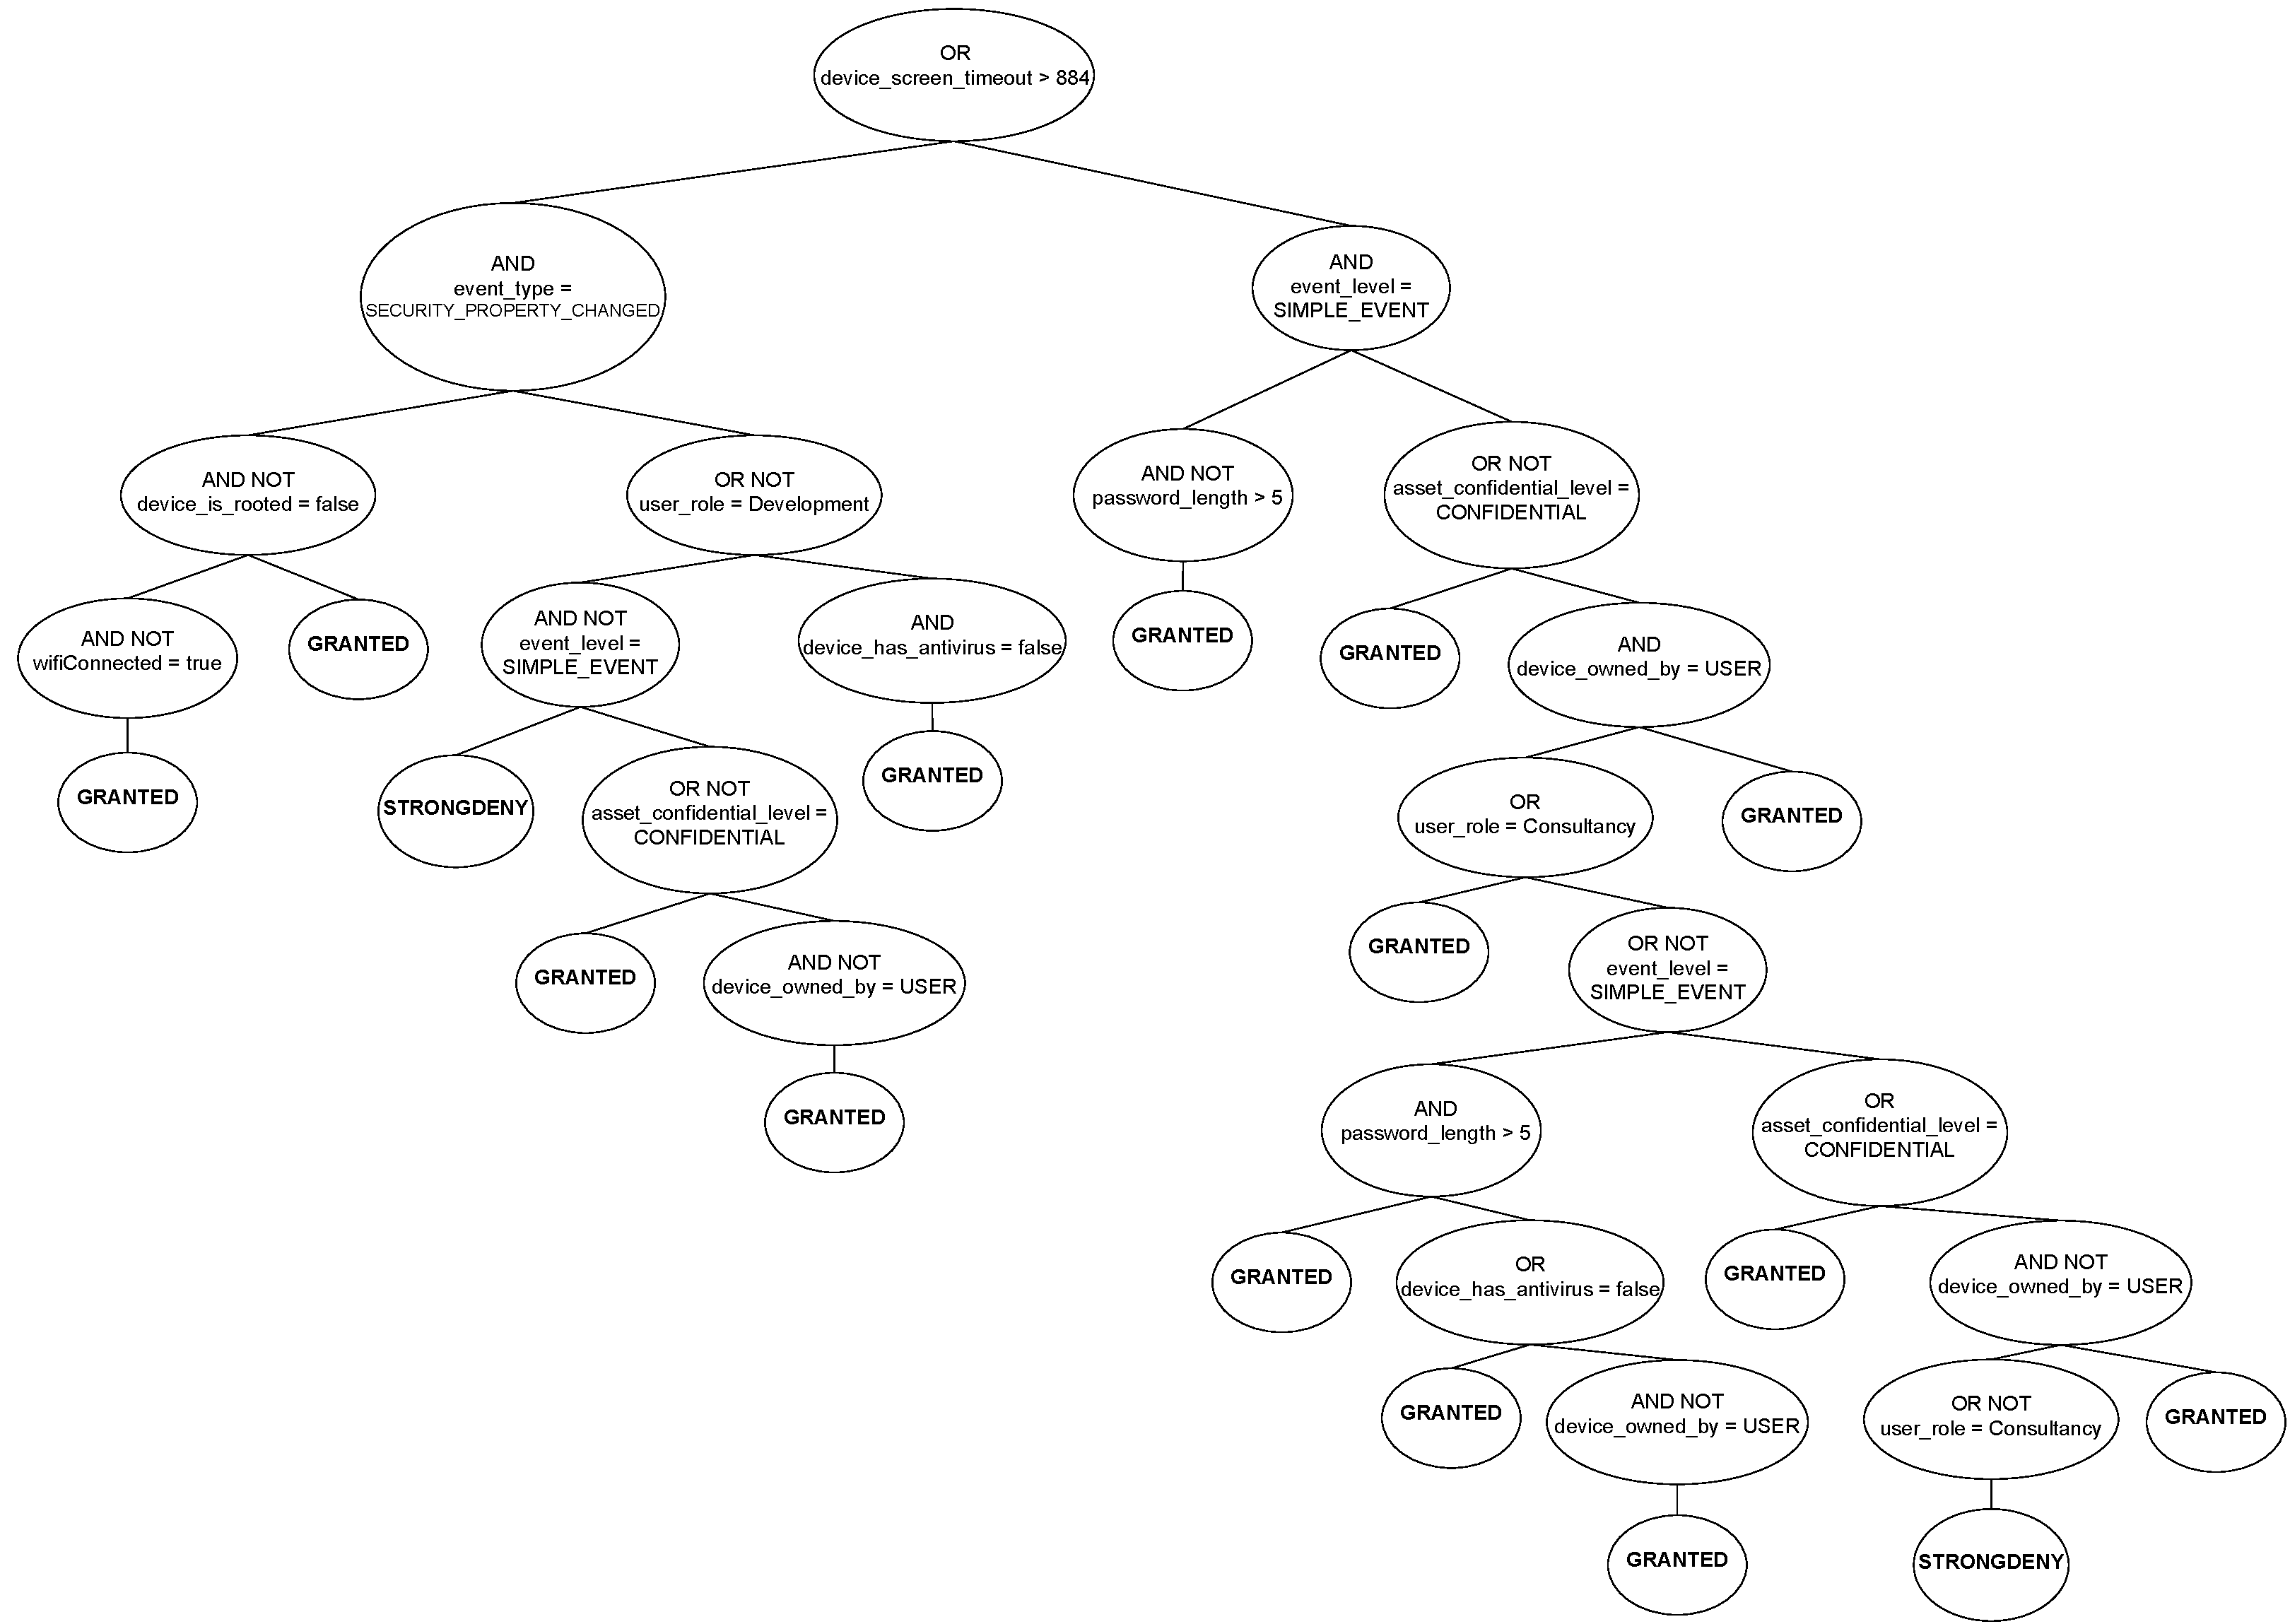
\includegraphics[width=0.8\textwidth]{img/bestInd_fCS_a0.pdf}
	\caption{An example of best individual obtained when using
          $f_{CS}$ as the fitness function with an $\alpha$ value of
          0. This tree represents a set of 16 rules, two of them
          classifying to the STRONGDENY class, whilst the rest
          classify towards the GRANTED class.} 
	\label{fig:bestInd_fCS_a0}
\end{figure*}

The STRONGDENY rules in Figure \ref{fig:bestInd_fCS_a0} imply that the developers are more probably to get a GRANTED in their actions, and this conclusion makes sense because because they are supposed to be more familiar with system security. Also, from the second rule we can infer that the complex events -- not simple -- and the devices owned by the users and not the company may be dangerous. The root condition, which appears in every rule and therefore means is very important, is related to the time that the the device takes to enter into sleep mode (screen turns off). This kind of information can be used by the CSOs to develop new security rules for the system.

In general, what we have seen in the individuals obtained by the
Pittsburgh approach is that most of the rules in the set classify for
the GRANTED class, and less than 13\% are classifying for the
STRONGDENY class. Again, the effect of the imbalance in the dataset is
present. Actually, in some cases the set of rules only classify to
GRANTED, and this can be seen as a ``whitelist'', meaning that
everything that is not specify by these rules will be automatically
denied.

%Maybe some comment on the root rule, which is the most discriminating
%one. Or some insight from the rules you could give the CSO - JJ

\section{Conclusions and Future Work}
\label{sec:future}

% General layout of conclusions
% We wanted to do this with this motivation.
% We have done this and that in this paper and met objective 1 and 2 or answered research question 1 and 2; however, we think that question 3 has not been answered properly
% We think we could answer question 3 properly if we did this and that. Which is left as future work.

In this work, we wanted to help companies adopting the BYOD philosophy
by developing a tool that is able to discover rules using a GP
approach, from the users behaviour when interacting with their
devices, at the time it minimises the false positives, so that a
dangerous action is never taken as permitted. To this end, in Section \ref{sec:methodology} we have
presented different ways to implement a methodology based on GP, by two
approaches: Pittsburgh, in which the individuals are coded as set or
rules; and Michigan, where the individuals are a single rule, and thus
a rule for every class has to be generated. In addition, two different
fitness functions have been used to study their effect over the
validation accuracy rate and the number of false positives and
negatives.

The results in Section \ref{sec:gp} make a fine proof of concept of a tool that helps the CSO of a company discovering dangerous situations through the presentation of GP generated rules. We obtained promising rates for the number of false positives (around
7\%), and good coverage over the validation data set is shown in Section \ref{subsec:approachcomparison}. However, since the ideal value for both false positives and negatives is 0, there is room for improvement. In addition, in section \ref{subsec:examples} we show that the individuals are presented in a readable form, but the ratio between rules classifying to one or another class is too much biased towards the GRANTED class. 

With regard to the execution time, the solution we propose takes between 16 and 17 hours, in the worst case and taking into account the used infrastructure, to obtain the best individual. Although these times could be acceptable, in the sense that the CSO would have new rules everyday, they can still be reduced.  
                                % Was it a challenge for GP? In which
                                % way?
                                % (Paloma) Yes? Maybe? Hope so? I don't know :( Pablo what do you think? 
% What follows is future work %Pablo: yes, I would move this paragraph at the end, and maybe add again the references you mentioned earlier in section 4.2
A possible way to
achieve better values for FP and FN is to set up the problem as a
multiobjective one, so that we try to minimise $f_{CS}$, but also FP
and FN. Additionally we will try to reduce the execution time by adapting the algorithm parameters, for instance, the number of generations, as has been shown in Section \ref{subsec:fitnesscomparison} that in some cases 50 generations is enough. Other enhancements could be to study every tree individual and to directly not evaluate the fitness for the contradictory rules of each one. 

On the other hand, the imbalance of the dataset should be taken into
account, given that it affects to the results in terms of obtained
accuracy in the validation process and the ratio among classes in the
obtained individuals. Solutions can be found in literature in order to reduce the bias while performing classification
tasks, such as in \cite{chawla2005data} and \cite{sun2009classification}. Another typical way of approaching this problem is to
use balancing techniques over the data, such as ``oversampling'' \cite{smote_02}, in
which sintetic instances of the minority class -- STRONGDENY -- are
created and introduced in the dataset, until there are approximately
the same number of instances than in the majority class -- GRANTED
--. Also, in \cite{bhowan2012developing}, the authors present a comparison between many different types of
fitness functions, testing on various unbalanced datasets, with
different minority-class/majority-class ratios.

For our future work we will implement these solutions to continue
improving our system. Furthermore, we will extend the approach to other problems where data is available. For example, particularisations of the BYOD problem as it could be Internet navigation during work hours. We will explore network traffic from public data repositories, such as \url{http://www.secrepo.com/#3p\_network}, and try to apply our approach. 

\section*{Acknowledgments.}

This work has been supported in part by TIN2014-56494-C4-3-P (Spanish
Ministry of Economy and Competitivity), PROY-PP2015-06 (Plan Propio
2015 UGR), and European project MUSES (FP7-318508). 

\bibliographystyle{elsarticle-num}
\bibliography{GPrules,geneura}

\end{document}
